\documentclass[a4paper,UTF8]{paper}
\usepackage{ctex}
\usepackage{amsmath}
\usepackage{pdfpages}
\usepackage{graphicx}
\usepackage{wrapfig}
\usepackage{listings}
\usepackage{multicol}
\usepackage{color}
\usepackage{alltt}
\usepackage{marvosym}
% Style definition file generated by highlight 3.6, http://www.andre-simon.de/ 

% Highlighting theme: Print 

\newcommand{\hlstd}[1]{\textcolor[rgb]{0,0,0}{#1}}
\newcommand{\hlnum}[1]{\textcolor[rgb]{0,0,0}{#1}}
\newcommand{\hlesc}[1]{\textcolor[rgb]{0,0,0}{#1}}
\newcommand{\hlstr}[1]{\textcolor[rgb]{0,0,0}{#1}}
\newcommand{\hlpps}[1]{\textcolor[rgb]{0,0,0}{#1}}
\newcommand{\hlslc}[1]{\textcolor[rgb]{0.4,0.4,0.4}{\it{#1}}}
\newcommand{\hlcom}[1]{\textcolor[rgb]{0.4,0.4,0.4}{\it{#1}}}
\newcommand{\hlppc}[1]{\textcolor[rgb]{0,0,0}{\bf{#1}}}
\newcommand{\hlopt}[1]{\textcolor[rgb]{0,0,0}{\bf{#1}}}
\newcommand{\hllin}[1]{\textcolor[rgb]{0.53,0.53,0.53}{#1}}
\newcommand{\hlkwa}[1]{\textcolor[rgb]{0,0,0}{\bf{#1}}}
\newcommand{\hlkwb}[1]{\textcolor[rgb]{0,0,0}{\bf{#1}}}
\newcommand{\hlkwc}[1]{\textcolor[rgb]{0,0,0}{\bf{#1}}}
\newcommand{\hlkwd}[1]{\textcolor[rgb]{0,0,0}{\bf{#1}}}
\definecolor{bgcolor}{rgb}{1,1,1}


\newcommand{\tabincell}[2]{\begin{tabular}{@{}#1@{}}#2\end{tabular}}
\begin{document}
\tableofcontents
\clearpage
\section{程序架构}
我们采用C++/Qt来开发现行平台,平台的核心是一个Traffic\_v1对象,如图\ref{UML}所示。

\begin{figure}
\centering
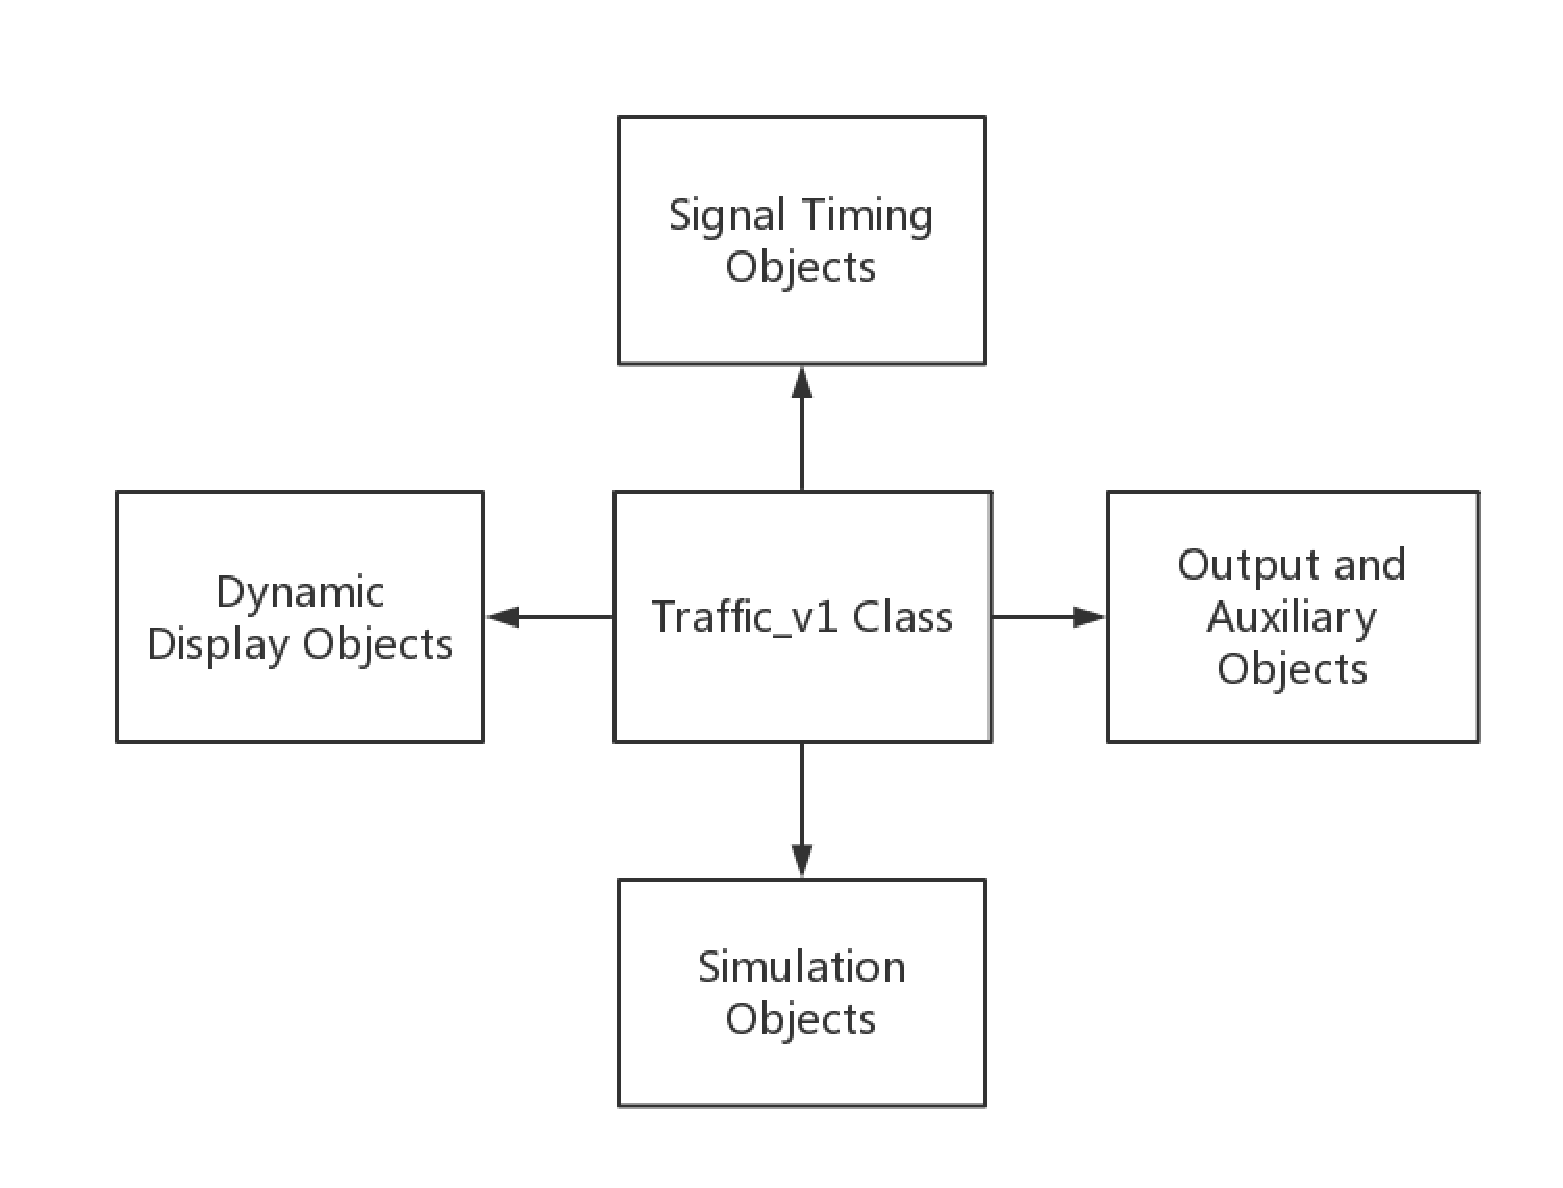
\includegraphics[width=\textwidth]{Diagram.eps}
\caption{Traffic\_v1 类的架构}
\label{UML}
\end{figure}

\subsection{显示模块}
这些模块用来动态显示仿真过程和控制仿真执行的流程,如设置仿真速度等。主要包括按键,标签,滑动条等对象。

当仿真每向前执行一步的时候,平台将刷新仿真模块来显示仿真过程中的具体情况,整个函数将完成如下几个步骤。

\begin{enumerate}
\item 绘制交通路口的基本要素

根据信号配时模块给出的信号相位,显示模块将绘制红绿灯。同时,显示模块将绘制交通路口前的车道,目前设定绘制30m长,22.5m宽的车道

\item 绘制车辆

绘制模块将绘制即将进入路口的车辆和驶离路口的车辆,在所有的车辆中,即将驶入路口的车辆是接受控制的,而驶离路口的车辆是不接受控制的,平台将为他们补全整个的控制策略。

\item 绘制交通路口中的车辆轨迹线

平台不处理车辆在交通路口内的行为,因此采用绘制车辆在路口中的轨迹线来表示车辆可能存在的位置。当车辆驶入交通路口时,我们假设左转车辆在交通路口的滞留时间是3s,而执行车辆在交通路口内的滞留时间是2s,右转车辆在交通路口内的滞留时间是1s,这些参数可以通过平台代码中的参数简单的修改。在滞留时间内的车辆会在交通路口内显示一道轨迹线,表示车辆可能在的位置。

可以看出,轨迹线的交点多少可以表示交通路口的混乱程度,如果交通路口内存在着大量的轨迹线交点,交通效率将受到影响,同时交通危险性将显著提升。而这一部分应当是信号配时的主要工作。
\end{enumerate}

\subsection{仿真模块}
这是整个平台的核心模块,通过设置的仿真速度,平台给出一个间隔为1ms(高速模式),10ms(中速模式),100ms(低速模式),1000ms(调试模式)的信号。

当触发信号被接受时,平台将按照如图\ref{int}所示的行为进行相关的操作。

\begin{figure}
\centering
\includegraphics[width=\textwidth]{TimeFlow.png}
\caption{平台执行流程}
\label{int}
\end{figure}

在执行过程中,进程控制模块根据用户设定的停止条件决定是否终止仿真,之后,每个道路的入口将根据车辆生成算法来生成新的车辆。之后,用户策略将根据车辆类型的不同分别和用户选择的模式应用在不同的车辆上。同时系统策略负责离开交通路口的车辆的行为和诸如进入交通路口等边界情况的处理。

所有的策略均调整车辆的加速度,在运动学仿真模块,平台将通过车辆现有的位置,速度和加速度计算车辆下一时刻的位置和速度。

最后,平台将处理进入交通路口的车辆和即将离开研究路段的车辆的边界情况。

程序之后完成界面的重绘工作,并等待下一个触发信号的到来。

根据现行平台实现,在一般配置的笔记本电脑上,在10ms的仿真时钟间隔的情况(中速模式)下系统压力还是比较合适的,同时平台产生的仿真数据也是比较合理的。当仿真时钟间隔被调整到1ms(高速模式),在交通压力过大的情况下会出现时序问题。

\subsection{输出和辅助模块}
这部分模块的主要作用是在系统重绘时或一些特殊情况发生时输出仿真结果。

随着仿真的进行,系统在可执行文件所在目录根目录中建立文件夹"result",在此文件夹内建立包含4张CSV表,一个子文件夹,这个子文件夹的命名规则是

\centerline{\textbf{'日期+时间+仿真模式选择'}}

四张CSV表中保存记录了不同类型的数据。

\begin{enumerate}
\item car.csv

这张表保存记录了车辆的初始速度(init\_velocity),理论到达时间(thoritical\_time) 和实际到达时间(act\_time), 理论到达时间被定义为车辆以最大加速度加速到最大速度之后进行匀速直线运动到达路口所花的时间。 理论到达时间 thoritical\_time 和实际到达时间 act\_time之间的差异可以描述车辆经过这段区域所浪费的时间。

\item stop.csv

这张表保存记录了每个车道上车辆的总停车次数和总共路口车辆的停车次数以及停车次数占整个车辆数量的比例。

\item road.csv

这张表记录了每个时刻驶离某一车道的车辆数量和离开系统的车辆数量,和相对应的平均值,这张表往往被用来检查仿真的合理性。

\item stop\_time.csv

这张表记录了每个车道上的总共的停车时间和整个系统内的通车时间以及分担到每个车辆上的停车时间。
\end{enumerate}

总的来说,road.csv 被用来观察 仿真过程是否正常执行而其他三个表用来评价整个所采用的驾驶策略的效率

另外,停车行为由车辆速度低于某个阈值决定,同时,当车辆停下时,停车时间不断累加,而停车次数不发生变化。这一点在长期停车时尤其明显。

\subsection{信号配时模块}

信号配时模块满足了用户自主设置信号周期和相位的要求,三个按键'set red behind'、 'set green behind'、 'set yellow behind' 被用来设置黑色时间线之后的信号相位。

同时,这个界面可以用来调整信号的周期。因此,通过调整黑色时间线或指定确定的调整时间,不断重复设置时间线之后的信号相位等工作,用户可以完全自主的完成信号的配时工作。

同时,左侧的界面将显示当前交通路口车辆的轨迹线,当前时间是黑色轨迹线所指示的时间。通过交通轨迹线的显示和对交叉情况的判断,系统可以在一定程度上辅助用户完成更好更合理的交通信号配时工作。
\subsection{平台界面}

仿真模块的界面和信号配时的界面如图\ref{cap1} 和图\ref{cap2}所示。

\begin{figure}
\centering
\includegraphics[width=\textwidth]{cap1.jpg}
\caption{仿真模块界面}
\label{cap1}
\includegraphics[width=\textwidth]{cap2.jpg}
\caption{信号配时模块的界面}
\label{cap2}
\end{figure} 

在仿真模块界面上点击'Edit Traffic Light'按钮可以激活信号配时模块的界面,如果用户关闭信号配时模块界面,他所作的变更将被保存同时仿真模块界面将被再次激活。

\clearpage
\section{算法简介}
\subsection{基础假设和参数}
首先,我们认为对车辆而言,车辆的加速度是可控的物理量,同时,其他的物理量(如速度和位置)由车辆的加速度和当前时刻的速度根据如下运动学公式确定: 
$$v(t+\Delta_t)=v(t)+a\Delta_t$$
$$x(t+\Delta_t)=x(t)+v(t)\Delta_t+0.5a\Delta_t^2$$ 

另外,由于车辆的加速度也不能被准确的控制,我们在策略给出加速度的准确值之后加入了一个正态分布的随机噪声,尤其是后文提到的人工驾驶的车辆模型,引入的正态分布随机噪声更大。

同时,平台对车辆的加速度和速度也有着限制,我们认为车辆加速度的绝对值的最大值是$a_{max}$,被用来限制车辆的加速过程和刹车过程。另外,车辆的最大速度被限制为$v_{max}$,车辆的最低速度被限制为$v_{min}$。

不论选择了那种驾驶策略,如果策略给出的加速度值大于最大加速度$a_{max}$或者小于$-a_{max}$,抑或是计算得到的速度大于最大速度或小于最小速度,程序将自动将这些值设定为对应的边界值。如果车辆受到红灯影响而被迫刹车停车,最小速度限制将被设定为0来描述可能的停车行为。但不论如何,倒车行为是永远不可接受的。

同时我们假设车辆期望的速度,$v_{exp}$,被设定为车辆最高限速的80\%。

为了简化模型,我们认为在所研究路段进行驾驶的过程中,车辆不进行变道行为。这个假设在现实情况中也是可以被接受的,因为受到交通法规和规则的限制,车辆在交通路口前的变道行为往往是被禁止或限制的。车辆需要在进入交通路口之前完成相关的变道工作,因此我们的假设是合理的,同时仅仅从交通效率的角度来看,换道行为也只能降低交通效率,不利于对驾驶策略进行评估。因此,因为平台的评估主要以策略为主,就不考虑车辆的换道行为了。

因此,在一个车道进行驾驶的车辆可以被描述成一个队列结构,即$Q_{in}$。

\subsection{车辆产生算法}
我们假设车辆的到达过程是一个泊松过程,这个到达过程受到下面算法的限制。

我们假设泊松过程的强度是$\lambda$到达车辆而定时间间隔$S_n,S_{n-1}$可以被表述为 
$$P((S_n-S_{n-1}\le t) = 1 - e^{-\lambda t}$$
因为仿真过程的时间间隔被设定为0.1s,每小时的平均车流量即为$$\bar{F}=36000\lambda$$

对于一个方向的车辆,车辆的小时流量被仿真界面上的交通流控制滑块设定之后,这个方向的车流量将按照特定的泊松过程进行生成$\lambda=\displaystyle{\frac{\bar{F}}{3600}}$, 并且被压入每个方向上的等待队列$Q_{pending}$。

在生成车辆之后,下一步是考虑车辆应当放入那个车道,我们认为车辆放入合理车道的可能性是相同的,合理车道被定义为车辆放入之后仍能安全行驶的车道。其具体定义可以被定义为,车辆生成位置($S_{start}$)和最后一个车辆的距离$X_{-1}$之间的距离大于安全行驶距离$S_{safe}$即,$$X_{-1}-S_{start}\le S_{safe}$$

遍历所有符合条件的合理车道,并且将$Q_{pending}$中的车辆等可能的放入其中的一条车道上。新生成的车辆的位置为$S_{start}$,即车辆生成线的位置。

如果目前没有合适的放入车辆的车道,车辆将被保留在$Q_{pending}$队列中并等待下一个仿真循环。

车辆生成的算法在整个仿真流程的第二步进行,紧随仿真流程控制模块。
\subsection{路口车辆排队的产生和消散}
\label{section:feq}
为了描述路口车辆排队的产生和消散过程,我们对每个驶入交通路口的车道引入队列$Q_{block}$。同时,根据现行信号相位和队列的长度,我们采用的所有控制策略几乎均采用如下提到的简单算法
\begin{enumerate}
\item 红灯

如果队列$Q_{in}$中的第一辆车辆和队列$Q_{block}$中的最后一辆车辆之间的距离小于控制距离$S_{control}$,队列$Q_{in}$中的第一个车辆将刹车并期望停在队列$Q_{block}$最后一辆车的期望距离之后。这个两车之间的期望距离被定义为$S_{stop}$,用来描述在队列$Q_{block}$中的车辆间距。 

If the $Q_{block}$ is empty and the distance between the first vehicle in $Q_{in}$ and the stopping line is less than $S_{control}$, the first vehicle in $Q_{in}$ brake and is expected to stop just on the stopping line$S_{end}$.

If the first vehicle in the $Q_{in}$is too far that neither of the two above are satisfied, the first vehicle in the $Q_{in}$ is supposed to drive freely.

Also, the vehicles in the $Q_{block}$ should stop and wait until the light truns green.
\item Green Light
distance between the first vehicle in $Q_{in}$ and the last vehicle in $Q_{block}$ (if it exists) should not be less than $S_{safe}$. And a braking is taken if the distance mentioned above is too short.
\end{enumerate}
Therefore, the brief idea of the algorithm above can be described as the fake code below\\ 

\noindent
\ttfamily
\hlstd{}\hllin{01\ }\hlkwa{if\ }\hlstd{}\hlopt{(}\hlstd{Q\textunderscore block}\hlopt{.}\hlstd{}\hlkwd{empty}\hlstd{}\hlopt{())\{}\\
\hllin{02\ }\hlstd{\ }\hlkwa{if\ }\hlstd{}\hlopt{(}\hlstd{Light\ }\hlopt{==\ }\hlstd{Green}\hlopt{)}\\
\hllin{03\ }\hlstd{}\hlstd{\ \ }\hlstd{Q\textunderscore in}\hlopt{.}\hlstd{}\hlkwd{first}\hlstd{}\hlopt{().}\hlstd{}\hlkwd{drive\textunderscore freely}\hlstd{}\hlopt{();}\\
\hllin{04\ }\hlstd{\ }\hlkwa{else}\\
\hllin{05\ }\hlstd{}\hlstd{\ \ }\hlstd{Q\textunderscore in}\hlopt{.}\hlstd{}\hlkwd{first}\hlstd{}\hlopt{().}\hlstd{}\hlkwd{brake\textunderscore to}\hlstd{}\hlopt{(}\hlstd{S\textunderscore end}\hlopt{);}\\
\hllin{06\ }\hlstd{}\hlopt{\}}\\
\hllin{07\ }\hlstd{}\hlkwa{else}\hlstd{}\hlopt{\{}\\
\hllin{08\ }\hlstd{\ }\hlkwa{if}\hlstd{}\hlopt{(}\hlstd{Q\textunderscore block}\hlopt{.}\hlstd{}\hlkwd{last}\hlstd{}\hlopt{().}\hlstd{pos}\hlopt{{-}}\hlstd{Q\textunderscore in}\hlopt{.}\hlstd{}\hlkwd{first}\hlstd{}\hlopt{().}\hlstd{pos}\hlopt{$<$\ }\hlstd{S\textunderscore control}\hlopt{)}\\
\hllin{09\ }\hlstd{}\hlstd{\ \ }\hlstd{Q\textunderscore in}\hlopt{.}\hlstd{}\hlkwd{first}\hlstd{}\hlopt{().}\hlstd{brake\textunderscore to\\
\hllin{10\ }}\hlstd{\ \ }\hlstd{}\hlopt{(}\hlstd{Q\textunderscore block}\hlopt{.}\hlstd{}\hlkwd{last}\hlstd{}\hlopt{().}\hlstd{pos}\hlopt{{-}}\hlstd{S\textunderscore stop}\hlopt{);\ }\\
\hllin{11\ }\hlstd{\ }\hlkwa{else}\\
\hllin{12\ }\hlstd{}\hlstd{\ \ }\hlstd{Q\textunderscore in}\hlopt{.}\hlstd{}\hlkwd{first}\hlstd{}\hlopt{().}\hlstd{}\hlkwd{drive\textunderscore freely}\hlstd{}\hlopt{();}\\
\hllin{13\ }\hlstd{}\hlopt{\}}\hlstd{}\\
\mbox{}
\normalfont
\normalsize


Where the brake\_to(desired\_pos) method means braking to a desired position.

Meanwhile, the growth and the dissipation of the queue $Q_{block}$ follow the method below.

\begin{enumerate}
\item Increase

If the first vehicle in $Q_{in}$ is closer than $S_{stop}$ from the last vehicle in $Q_{block}$ (it is set to $S_{end}$ if the $Q_{block}$ is empty), it is removed from the $Q_{in}$ and pushed into the $Q_{block}$

\item Dissipation

When the traffic light is green, all of the vehicles in the $Q_{block}$ is moving forward at the speed of $v_{dis}$, since the speed is relatively low, the acceleration process and any other phenomenon can be ignored. When the vehicle moves over the stopping lane and enters the intersection, it is removed from the $Q_{block}$
\end{enumerate}
And the method above can be described as the fake code below\\

\noindent
\ttfamily
\hlstd{}\hllin{01\ }\hlkwa{if\ }\hlstd{}\hlopt{(}\hlstd{light\ }\hlopt{==\ }\hlstd{green}\hlopt{)\{}\\
\hllin{02\ }\hlstd{\ Q\textunderscore block}\hlopt{.}\hlstd{}\hlkwd{all\textunderscore move\textunderscore forward}\hlstd{}\hlopt{(}\hlstd{v\textunderscore dis}\hlopt{)}\\
\hllin{03\ }\hlstd{}\hlopt{\}}\\
\hllin{04\ }\hlstd{}\hlkwa{else}\hlstd{}\hlopt{\{}\\
\hllin{05\ }\hlstd{\ }\hlkwa{if}\hlstd{}\hlopt{(!}\hlstd{Q\textunderscore block}\hlopt{.}\hlstd{}\hlkwd{empty}\hlstd{}\hlopt{())\{}\\
\hllin{06\ }\hlstd{}\hlstd{\ \ }\hlstd{}\hlkwa{if}\hlstd{}\hlopt{(}\hlstd{Q\textunderscore block}\hlopt{.}\hlstd{}\hlkwd{last}\hlstd{}\hlopt{().}\hlstd{pos}\hlopt{{-}}\hlstd{Q\textunderscore in}\hlopt{.}\hlstd{}\hlkwd{first}\hlstd{}\hlopt{().}\hlstd{pos\\
\hllin{07\ }}\hlstd{\ \ \ }\hlstd{}\hlopt{$<$\ }\hlstd{S\textunderscore stop}\hlopt{)\{}\\
\hllin{08\ }\hlstd{}\hlstd{\ \ \ }\hlstd{Vehicle\ v}\hlopt{;}\\
\hllin{09\ }\hlstd{}\hlstd{\ \ \ }\hlstd{v}\hlopt{=}\hlstd{Q\textunderscore in}\hlopt{.}\hlstd{}\hlkwd{getfirst}\hlstd{}\hlopt{();}\\
\hllin{10\ }\hlstd{}\hlstd{\ \ \ }\hlstd{Q\textunderscore block}\hlopt{.}\hlstd{}\hlkwd{push}\hlstd{}\hlopt{(}\hlstd{v}\hlopt{);}\\
\hllin{11\ }\hlstd{}\hlstd{\ \ }\hlstd{}\hlopt{\}}\\
\hllin{12\ }\hlstd{\ }\hlopt{\}}\\
\hllin{13\ }\hlstd{\ }\hlkwa{else}\hlstd{}\hlopt{\{}\\
\hllin{14\ }\hlstd{}\hlstd{\ \ }\hlstd{}\hlkwa{if}\hlstd{}\hlopt{(}\hlstd{S\textunderscore end}\hlopt{{-}}\hlstd{Q\textunderscore in}\hlopt{.}\hlstd{}\hlkwd{first}\hlstd{}\hlopt{().}\hlstd{pos}\hlopt{$<$\ }\hlstd{S\textunderscore stop}\hlopt{)\{}\\
\hllin{15\ }\hlstd{}\hlstd{\ \ \ }\hlstd{Vehicle\ v}\hlopt{;}\\
\hllin{16\ }\hlstd{}\hlstd{\ \ \ }\hlstd{v}\hlopt{=}\hlstd{Q\textunderscore in}\hlopt{.}\hlstd{}\hlkwd{getfirst}\hlstd{}\hlopt{();}\\
\hllin{17\ }\hlstd{}\hlstd{\ \ \ }\hlstd{Q\textunderscore block}\hlopt{.}\hlstd{}\hlkwd{push}\hlstd{}\hlopt{(}\hlstd{v}\hlopt{);}\\
\hllin{18\ }\hlstd{}\hlstd{\ \ }\hlstd{}\hlopt{\}}\\
\hllin{19\ }\hlstd{\ }\hlopt{\}}\\
\hllin{20\ }\hlstd{\ }\\
\hllin{21\ }\hlopt{\}}\hlstd{}\\
\mbox{}
\normalfont
\normalsize


All above describe the formation and evacuation of the queue in the intersection and its interaction with other models. The differences caused by the assumption can be ignored. Thanks to this model, it is easy for us to decouple the driving model and the queuing model, which makes it much easier to implement the other algorithm
\subsection{Basic models}
In the description of manual driving and automatic driving vehicle models, the car-following model and free driving model are frequently used models. Therefore, we will describe these models before discussing the control strategies.

\subsubsection{The implementation of the free-driving method}

When there is no speed guidance, a vehicle's driving behavior can be roughly classified into free-driving and car-following, which will be described in this section and the next section. $S_{control}$ is defined as the distance of interaction between vehicles. Thus, the two driving models are chosen according to the rules below.

\begin{enumerate}
\item When the distance to the front vehicle from the vehicle which we are concerned about is less than $S_{control}$, the driving choose the car-following strategy.

\item When the distance is greater than $S_{control}$, the driver choose the free-driving strategy, which means trying to reach the expected speed, $v_{exp}$, during this period, a smaller acceleration may be chosen if the current speed of vehicle is almost the same as $v_{exp}$, while a greater acceleration should be chosen if the current speed is too low, such as the vehicle is stopped.

Also, because some random noise may be introduced to the system, if the speed of the vehicle is higher than $v_{max}$, a minor deceleration should be taken.
\end{enumerate}
\subsubsection{The implementation of the car-following method}
\label{cf}

As mentioned above, when the vehicles is close enough to each other, the car-following method is chosen. In the strategy we used, the commonly used driving psycho-physical model—Wiedemann model is adopted, that is,
$$a_n(t+\Delta_t)=\frac{[\Delta v_{n,n-1}(t)]^2}{2[\Delta x_{n,n-1}(t)-S_{exp}]}+a_{n-1}(t)$$

In the above equation, $S_{exp}$ represents the expected minimum safe-following distance. Since the speed of the vehicle in the intersection may have a big range, $S_{exp}$ should not be a constant. Therefore, according to the regulations on safe distance in Regulation on the Implementation of the Road Traffic Safety Law of the People's Republic of China, we use the linear correlation model of the minimum safe following distance and the speed of the front vehicle, therefore, the $S_{exp}$ can be described like this,
$$S_n(t)=\alpha v_{n-1}(t)+S_{safe}$$
While the $S_{safe}$is the same as the distance between the vehicles in \ref{section:feq}, and the constant $\alpha$ may be set by according to the experience.

Once the distance between the vehicles is less than $S_{exp}$, which means the distance between the vehicles is too short, an emergency brake is taken owing to the specific situation. In most cases, the acceleration of the vehicle is set to $0.5a_{max}$
\subsection{Manual driving model}
\label{section:man}
The plantform provides three models to verify the effectiveness of the platform, and the first model is manual driving model.

As the name of the model indicates, manual driving model is used to describe the behavior of a vehicle driving by human. This model is often used to provide a 'basic' traffic efficiency, while other control strategies are expected to behave better than this simple model.

Firstly, vehicles which are far (greater than $S_{inter}$) from the intersection are taken into consideration. Because they are so far from the intersection, they do not consider the influence of the traffic light. 

Therefore, these vehicles mat take the car-following method or the free-driving method. If a vehicle is the first one in $Q_{in}$, it has to take the the free-driving method.

As for the ones which are closer to the intersection, different method will be chosen to meet the different situation below.

\begin{enumerate}
\item Green traffic light with an empty waiting queue $Q_{block}$

In this situation, the behavior of the vehicles is similar to the behavior described above.

In addition to the behavior mentioned, the remain time of the green light is calculated, if the remaining time is less than $T_{safe}$, the possibility of entering the intersection during the green light may be taken into consider, if it is difficult for the vehicle to pass the stopping line before the light turns red, the vehicle may behave like the traffic light is red.

\item Green traffic light while the  waiting queue $Q_{block}$ is not empty

During this situation, the vehicles discussed may brake or accelerate to set its speed to $v_{dis}$, and try to enter the queue $Q_{block}$, once it enters the $Q_{block}$, it will move with the other vehicles in the queue.

Also, if the remaining time is less than $T_{safe}$, the program may consider slow down the vehicle and prepare to stop. 
\item Red traffic light

In this case, the vehicles discussed will behave just like what we have discussed in \ref{section:feq}
\end{enumerate}

What's more, we focus on portraying the behavior of the first vehicle in the driving queue $Q_{in}$, since the vehicles behind it can be controled easily by car-following method.

Taking all of the situations into consideration. the manual driving model can be abstract as the fake code below.\\
 
\noindent
\ttfamily
\hlstd{}\hllin{01\ }\hlslc{//the\ code\ below\ just\ consider\ the\ vehicle\ v}\\
\hllin{02\ }\hlstd{}\hlkwa{if}\hlstd{}\hlopt{(}\hlstd{S\textunderscore end}\hlopt{{-}}\hlstd{v}\hlopt{.}\hlstd{pos}\hlopt{$>$}\hlstd{S\textunderscore inter}\hlopt{)}\hlstd{}\hlslc{//far\ from\ intersection}\\
\hllin{03\ }\hlstd{}\hlopt{\{}\\
\hllin{04\ }\hlstd{\ }\hlslc{//code\ block\ 1}\\
\hllin{05\ }\hlstd{\ }\hlkwa{if}\hlstd{}\hlopt{(}\hlstd{car}\hlopt{{-}}\hlstd{}\hlkwd{following\textunderscore requirement\textunderscore met}\hlstd{}\hlopt{())}\\
\hllin{06\ }\hlstd{}\hlstd{\ \ }\hlstd{}\hlslc{//the\ car{-}following\ requirement\ is}\hlstd{\ \ }\hlslc{met}\\
\hllin{07\ }\hlstd{}\hlstd{\ \ }\hlstd{}\hlkwd{car\textunderscore following}\hlstd{}\hlopt{();}\\
\hllin{08\ }\hlstd{\ }\hlkwa{else}\\
\hllin{09\ }\hlstd{}\hlstd{\ \ }\hlstd{}\hlslc{//the\ head\ car\ of\ the\ queue\ or}\\
\hllin{10\ }\hlstd{}\hlstd{\ \ }\hlstd{}\hlslc{//the\ car{-}following\ requirement\ isn't\ met}\\
\hllin{11\ }\hlstd{}\hlstd{\ \ }\hlstd{}\hlkwd{free\textunderscore driving}\hlstd{}\hlopt{();}\\
\hllin{12\ }\hlstd{}\hlopt{\}}\\
\hllin{13\ }\hlstd{}\hlkwa{else\ }\hlstd{}\hlslc{//close\ to\ the\ intersection}\\
\hllin{14\ }\hlstd{}\hlopt{\{\ }\\
\hllin{15\ }\hlstd{\ }\hlkwa{if}\hlstd{}\hlopt{(}\hlstd{light}\hlopt{==}\hlstd{red}\hlopt{)}\\
\hllin{16\ }\hlstd{}\hlstd{\ \ }\hlstd{method1}\hlopt{.}\hlstd{}\hlkwd{3}\hlstd{}\hlopt{();}\hlstd{}\hlslc{//the\ method\ mentioned\ in\ 1.3}\\
\hllin{17\ }\hlstd{\ }\hlkwa{else}\\
\hllin{18\ }\hlstd{}\hlstd{\ \ }\hlstd{}\hlkwa{if}\hlstd{}\hlopt{(}\hlstd{Q\textunderscore block}\hlopt{.}\hlstd{}\hlkwd{empty}\hlstd{}\hlopt{())\{}\\
\hllin{19\ }\hlstd{}\hlstd{\ \ \ }\hlstd{}\hlkwa{if}\hlstd{}\hlopt{(}\hlstd{time\textunderscore remain}\hlopt{$>$}\hlstd{T\textunderscore safe}\hlopt{)}\\
\hllin{20\ }\hlstd{}\hlstd{\ \ \ }\hlstd{}\hlslc{//same\ as\ the\ code\ block\ 1}\\
\hllin{21\ }\hlstd{}\hlstd{\ \ \ }\hlstd{}\hlkwa{else\ }\\
\hllin{22\ }\hlstd{}\hlstd{\ \ \ \ }\hlstd{}\hlkwa{if}\hlstd{}\hlopt{(!}\hlstd{}\hlkwd{pass\textunderscore check}\hlstd{}\hlopt{())}\\
\hllin{23\ }\hlstd{}\hlstd{\ \ \ \ }\hlstd{}\hlslc{//same\ as\ the\ red\ light\ case}\\
\hllin{24\ }\hlstd{}\hlstd{\ \ \ }\hlstd{}\hlopt{\}}\\
\hllin{25\ }\hlstd{}\hlstd{\ \ }\hlstd{}\hlkwa{else}\\
\hllin{26\ }\hlstd{}\hlstd{\ \ \ }\hlstd{}\hlkwa{if}\hlstd{}\hlopt{(}\hlstd{time\textunderscore remain}\hlopt{$>$}\hlstd{T\textunderscore safe}\hlopt{)}\\
\hllin{27\ }\hlstd{}\hlstd{\ \ \ }\hlstd{}\hlkwd{acc\textunderscore to\textunderscore speed}\hlstd{}\hlopt{(}\hlstd{v\textunderscore dis}\hlopt{);}\\
\hllin{28\ }\hlstd{}\hlstd{\ \ \ }\hlstd{}\hlkwa{else\ }\\
\hllin{29\ }\hlstd{}\hlstd{\ \ \ \ }\hlstd{}\hlkwa{if}\hlstd{}\hlopt{(!}\hlstd{}\hlkwd{pass\textunderscore check}\hlstd{}\hlopt{())}\\
\hllin{30\ }\hlstd{}\hlstd{\ \ \ \ }\hlstd{}\hlslc{//same\ as\ the\ red\ light\ case}\\
\hllin{31\ }\hlstd{}\hlstd{\ \ \ }\hlstd{}\hlopt{\}}\\
\hllin{32\ }\hlstd{}\hlstd{\ \ }\hlstd{}\\
\hllin{33\ }\hlopt{\}}\hlstd{}\\
\mbox{}
\normalfont
\normalsize


The plantform will traverse the queue $Q_{in}$, and during each iteration, the acceleration of the vehicle in processing will be set according to the model given above.

\subsection{The single-vehicle cooperative speed guidance model}
\label{section:st1}
Applied some changes on the car-following strategy, we designed a cooperative speed guidance model which only takes the influence of the traffic light into consideration.
\subsubsection{Modification about the car-following method}
Firstly, when the distance to the front vehicle from the vehicle which we are concerned about is less than $S_{control}$, the car-following model in chosen. In addition to the basic car-following method, it is changed to the following form when $\Delta x_{n,n-1}(t)\le S_{exp}$ 
$$a_n(t+\Delta_t)=-sgn(\Delta v_{n,n-1}(t))\frac{[\Delta v_{n,n-1}(t)]^2}{2[\Delta x_{n,n-1}(t)-S_{exp}]}+a_{n-1}(t)$$
which means, if the speed of the following vehicle is lower, the strategy will suggest that this vehicle should accelerate.

With this minor modification, some experimental researches show that the changed car-following method works well and can keep a stable distance between the vehicles.

As the fig.\ref{carf} shows, the vehicle following takes the modified car-following method and the front vehicle decelerate with a large random noise. From the figure it can be found that the distance between these two vehicles will be stable near $S_{exp}$, no matter what initial situation is chosen.
\begin{figure}
\centering
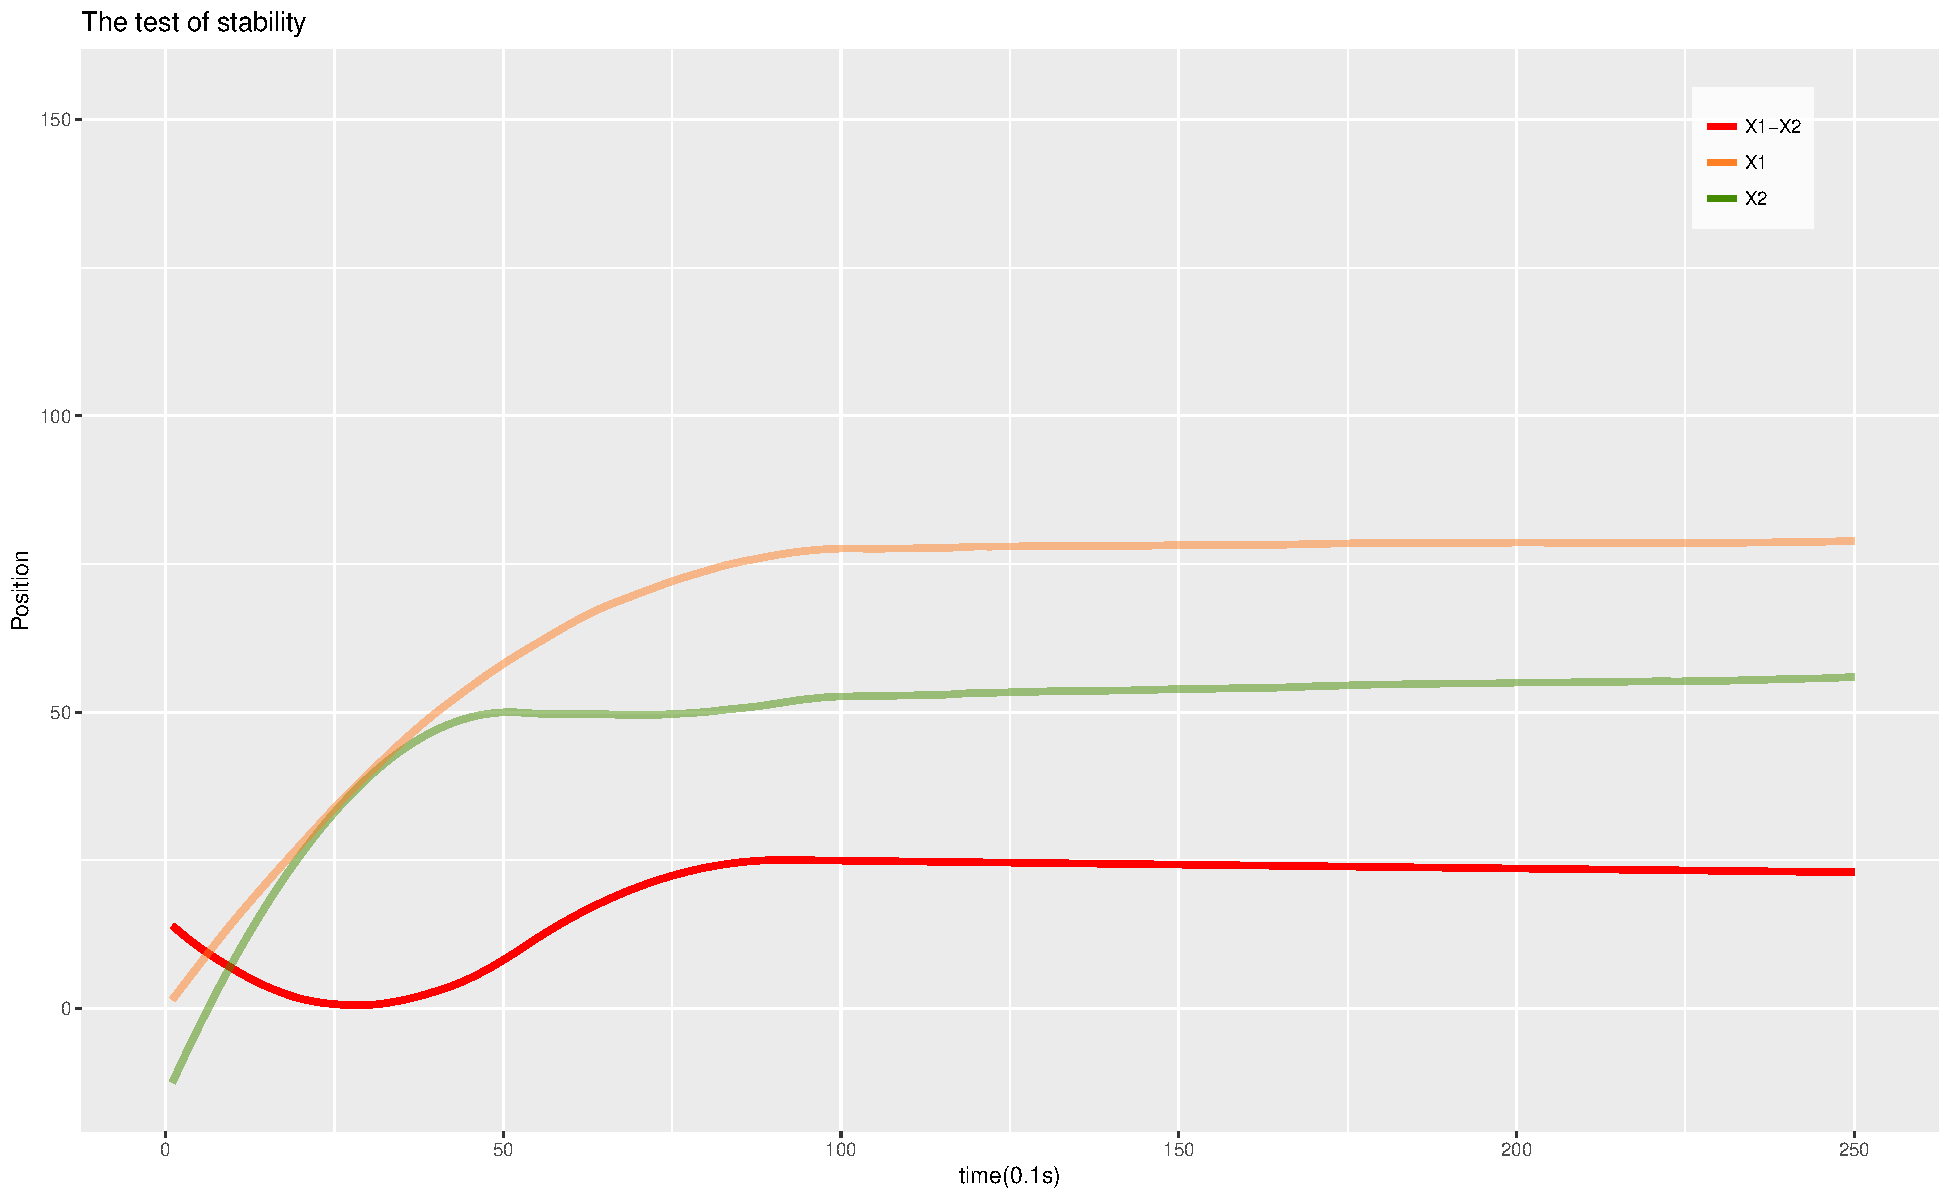
\includegraphics[width=\textwidth]{NearlyGoDie_2.pdf}
\caption{The position of the vehicles and the distance between them}
\label{carf}
\end{figure}
\subsubsection{The cooperative vehicle strategies}
\label{section:tgs}
Besides the chaning on car-following method, the free-driving model is also replaced by the following cooperative vehicle strategy. 

First of all, we define two parameters, the maximum time cost $T_{max}$ is defined as the time cost if the vehicle firstly decelerates at the acceleration of $-a_{max}$ and maintain a uniform linear motion at the speed of $v_{min}$ until it reaches the intersection. Also, the minimum time cost $T_{min}$ is defined as the time cost if the vehicle firstly accelerates at the acceleration of $a_{max}$ and maintain a uniform linear motion at the speed of $v_{max}$ until it reaches the intersection. It is obvious that the actual time cost of a vehicle is less than $T_{max}$ and greater than $T_{min}$, and both the $T_{max}$ and the $T_{min}$ depengs only on the initial speed $v_{init}$ of the vehicle starting from the start line.

Then, the strategy determines the earliest green time $T_G$ in the interval $(T_{min},T_{max}]$ with the accuracy in second. If there is no green time during this interval, a free-driving strategy is applied to the vehicle.

If a proper $T_G$ could be set, an acceleration or a deceleration may be applied to the vehicle to adjust its motion at the aim of reaching the stopping line at the time of $T_G$. During this period, if the vehicle is affected by the preceding vehicle, the car-following model may be applied to the vehicle again.

Meanwhile, the behavior the vehicle takes is similar to the one in the manual driving method.

Generally speaking, this strategy is the optimize version of the car-following model with the consideration of the influence of the traffic light.
\subsection{The multi-vehicle cooperative speed guidance model}
\label{section:st2}
This is a simple connect-vehicle strategy with the communication between the vehicles.

The strategy is operated from the first vehicle in $Q_{in}$ to the last vehicle in $Q_{in}$

First of all, the first vehicle in $Q_{in}$ determine its arrival time $T_G$ according to the method mentioned in section \ref{section:tgs}, and we set the $T_G$ determined by the n-th vehicle in $Q_{in}$ is $T_G^{[n]}$, e.g. the first vehicle determines $T_G^{[1]}$

After chosing the $T_G^{[1]}$, an acceleration or a deceleration may be applied to the vehicle to adjust its motion at the aim of reaching the stopping line at the time of $T_G^{[1]}$, if the $T_G{^[1]}$ does not exist, the vehicle takes an acceleration and then stops at the stopping line.

Then, it is assumed that the [n+1]-th vehicle in $Q_{in}$ can acquire the $T_G^{[n]}$ of the n-th vehicle in $Q_{in}$, including whether it exists.

The [n+1]-th vehicle determins its $T_G^{[n+1]}$according to its $T_{min}$ and $T_{max}$ and make sure that the $T_G^{[n+1]}-T_G^{[n]} \ge 1 \mathrm{second}$, owing to the fact that the following vehicle is supposed to arrive later than the preceding vehicle.

If the $T_G^{[n]}$ does not exist, $T_G^{[n]+1}$ should be set freely, only depends on the $T_{max}$ and the $T_{min}$ of the vehicle.

Then the acceleration of the [n+1]-th vehicle is set according to the expected time of arrival. The strategy then goes for the following vehicles.

Since the expected time of arrival is carefully designed to make sure that the following vehicle always arrives the stopping line later than the preceding vehicle, even the vehicles which do not have an expected arrival time will take an acceleration, the probability of the rear-ending is minor, a rear-ending will be solve by some simple emergency settings. 
\subsection{The processing of the strategies and the combination of the strategies}
\subsubsection{Single strategy simulation}
The plantform treats the strategies as an iteration from the last vehicle in the $Q_{in}$ to the first one in that, for the reason that the following vehicles may acquire the acceleration of the preceding car which should be fixed until the acceleration is set according to the strategy chosen by user. 

Therefore, if only a specific strategy is chosen, the program behaves like a loop from the last to the first of $Q_{in}$.

\subsubsection{Combination of the strategies}
Only the combination of the manual driving vehicle and the speed guidance models are concerned about, therefore, the plantform only include two kinds of combination simulation, which is the combination between the manual driving vehicle(mentioned in \ref{section:man}) and the single-vehicle cooperative speed guidance model (mentioned in \ref{section:st1}); and the combination between the manual driving vehicle and the multi-vehicle cooperative speed guidence model (mentioned in \ref{section:st2})

During the vehicle generating step, the control strategy of the vehicle is set by random method according to the type of combination and the ratio set by user.

After generate the type of the control strategy, the user-strategy step of the simulation set the acceleration of the vehicle using the strategy it has. It is assmued that if a vehicle using multi-vehicle cooperative speed guidence model is following a manual driving vehicle, the expected arrival time of the manual driving vehicle $T_G$ does not exist, therefore, the speed guidence model could set its expected arrival time $T_G$ freely.

\subsection{Add on algorithms}
Besides this, some add on algorithm is added to treat some accidents may happen accidentally. And the implementations of these specific algorithms may be found in the code of the plantform.
\end{document}